\section{Implementation}
\label{sec:impl}

\Egglog is implemented in approximately 4,200 lines of Rust~\cite{rust}.
The codebase is open-source.\footnote{\url{https://github.com/mwillsey/egg-smol}.}
\Egglog provides both a library interface 
 and the text format shown in \autoref{sec:overview}.
As suggested by the previous sections,
 \egglog's design and implementation takes
 many cues from modern Datalog implementations~\cite{souffle,ascent,inca}.
Below, 
 we describe the design of \egglog's core components,
 as well as some of the benefits of this design.

\subsection{Components}\label{sec:components}

\Egglog's main components are 
 the database itself,
 rebuilding procedure,
 and the query engine.

\paragraph{Database}
Unlike most other Datalog implementations,
 \Egglog is based on a functional database instead of a relational database.
In other words, 
 each function/relation is backed by a map instead of a set.
This ensures that \Egglog can efficiently 
 perform the ``get-or-default'' operation required to implement terms.
For example,
 evaluating the term \lstinline{(g x)}
 will first lookup \lstinline{x} in the map for function \lstinline{g}.
If something is present, 
 it will be returned,
 otherwise \lstinline{g}'s 
 \lstinline{:default} expression is evaluated,
 placed in the map for \lstinline{(g x)},
 and returned.

The functional database also ensures that 
 a function's inputs map to a single output.
As discussed in \autoref{sec:merge},
 \egglog uses a function's \lstinline{:merge} expression
 to resolve conflicts in map.
Function conflicts can arise in two ways:
 (1) the user or a rule expressly calls 
 \lstinline{(set (f x) y)} where \lstinline{(f x)} is already defined,
 or 
 (2) a \lstinline{union} causes a function's inputs to become equivalent.
The functional database allows for efficient detection of the first case;
 the second essentially requires computing congruence closure,
 which is done by the rebuilding procedure.

\paragraph{Rebuilding Procedure}

\Egglog's rebuilding procedure is based on 
 the rebuilding procedure from \egg~\cite{egg},
 which is in turn based on the congruence closure algorithm from \citet{tarjan-congruence}.
The rebuilding procedure is responsible for
 canonicalizing the database,
 which resolves (and creates)
 the second form of function conflicts discussed above.
Suppose that a function 
 $f$ maps two different inputs to two different outputs:
 so $f(a) \mapsto b$ and $f(c) \mapsto d$.
Say that $a$ and $c$ have recently been \lstinline{union}ed,
 and that $a$ is canonical;
 rebuilding must update the entry $f(c) \mapsto d$,
 since it is no longer canonical.
Canonicalizing $f(c) \mapsto d$
 to $f(a) \mapsto d$
 causes a conflict with the previously existing entry $f(a) \mapsto b$.
To resolve conflicts,
 \egglog uses the \lstinline{:merge} expression
 to combine the two outputs into a single output.
The \lstinline{:merge} may end up \lstinline{union}ing more things,
 which may in turn create more conflicts.
The rebuilding procedure continues until
 no more conflicts are created.
For functions where the \lstinline{:merge} 
 behavior is to \lstinline{union} the two outputs,
 this is the same as congruence closure.
For other \lstinline{:merge} behavior,
 this is more akin to the \eclass analysis propagation algorithm
 from \citet{egg}.

\paragraph{Query Engine}

Once the database is canonicalized,
 \ematching is reduced to a query over the database.
Since \egglog is based on Datalog, 
 it can naturally use established techniques for efficient query execution.
\Egglog's query engine is based on 
 the relational \ematching technique from \citet{relational-ematching},
 which uses a worst-case optimal join algorithm called Generic Join~\cite{generic-join}.
\Egglog also features
 some important optimizations on top of \citet{relational-ematching}'s
 implementation
 that are only possible because of \egglog's database-native approach\footnote{
    \citet{relational-ematching}'s implementation still uses an \egraph
    data structure; 
    it creates a database from the \egraph whenever it needs to \ematch.
    \Egglog avoids this copying overhead since it is already a database.
 }, \revision{such as the \seminaive evaluation presented in \autoref{sec:seminaive}}
\revdel{
The most significant optimization is the \seminaive algorithm.
In essence,
 the \seminaive algorithm allows for running a Datalog program
 without re-discovering old facts.
In the path example in \autoref{fig:datalog-tc},
 the \naive approach re-discovers old paths every iteration, 
 but the \seminaive approach only discovers new paths.
The \seminaive algorithm
 works by splitting each relation (or function in \egglog)
 into a new and old portion.
When computing a query,
 the query engine can then ignore results 
 that do not reference any new tuple,
 since such results would have been found in a previous iteration.
}
% \revision{
% \Egglog also features
% some important optimizations on top of \citet{relational-ematching}'s
% implementation
% that are only possible because of \egglog's database-native approach.\footnote{
%     \citet{relational-ematching}'s implementation still uses an \egraph
%     data structure; 
%     it creates a database from the \egraph whenever it needs to \ematch.
%     \Egglog avoids this copying overhead since it is already a database.
% }
% The most significant optimization is the \seminaive algorithm from Datalog evaluation.
% In essence,
% the \seminaive algorithm allows for running a Datalog program
% without re-discovering old facts.
% % In the path example in \autoref{fig:datalog-tc},
% %  the \naive approach re-discovers old paths every iteration, 
% %  but the \seminaive approach only discovers new paths.
% \egglog uses the \seminaive algorithm similar to Datalog to effectively incrementalize the evaluation.
% The core observation of
% \seminaive for Datalog is that, at each iteration
% some new facts are introduced and all old facts
% are preserved.
% Therefore, when performing queries
% it suffices to join ``new with new''
% and ``new with old'',
% because any elements from ``old with old`` join must have been computed by a previous iteration.
% This same argument also holds for \egglog programs,
% although in \egglog we have to be more careful when we define ``new tuple''.

% % Like Datalog, a tuple is considered new 
% % if it was added in the last iteration of the rules.
% % However, in \egglog queries can depend on the equality of two ids in the database.
% % Therefore, a tuple is also considered new if 
% % its canonical representation changed in the previous iteration.
% % The correctness of \seminaive for \egglog follows via a similar induction to Datalog.
% % This holds even when the rules may be non-monotone, 
% % because the inflationary semantics of \egglog guarantees 
% % that old facts will not be removed in later iterations.
% }


\subsection{Language-based Design}

Like most Datalog implementations (and \emph{unlike} most \eqsat implementations),
 \egglog is designed primarily as a programming language.
Users can write \egglog programs in a text format 
 (shown in \autoref{sec:overview}),
 and the tool parses, typechecks, compiles, and executes them.
The \egglog language includes 
 several base types (including 64-bit integers and strings)
 and operations over them.
Users can also define their own types and operations
 by using the Rust library interface.

Compared to tools like \egg
 that are more embedded in the host language,
 this design provides more
 of the user's program to the compiler for 
 checking and optimization.
For example,
 \egg provides conditional rewrite rules
 that gate a rewrite on some condition. 
The guards are essentially Rust code,
 so \egg cannot inspect them;
 it must just run the query and then check the guard.
In \Egglog, 
 there is no need for special conditional rewrites;
 all rules (and therefore rewrites) 
 can have as many conditions in the query as needed.
In addition,
 rewrite rules in \egg are not typechecked;
 \egglog prevents common errors by statically typechecking rules.
The language-based approach also allows
 the user to better model their problem
 with as many datatypes, functions, and analysis as needed.
\egg is artificially limited 
 to a single type and a single analysis in the \egraph
 due to its embedded nature;
 allowing for multiplicity would 
 significantly complicate
 the generic types in \egg's Rust implementation.
 

\subsection{Micro-benchmarks}

\begin{figure}[]
    % \begin{minipage}[t]{0.45\linewidth} 
    %     \centering
    %     \begin{tabular*}{}[]{}
    %                     & \egg & \egglog \\
    %     \texttt{math} &    0.01s & 0.02s \\
    %     \texttt{lambda} &  0.48s & 0.05s \\
    %     \end{tabular*}
    %     \caption{TODO}
    %     \label{f2}
    % \end{minipage}   
    % \hfill
    % \begin{minipage}[t]{0.45\linewidth}
        \centering
        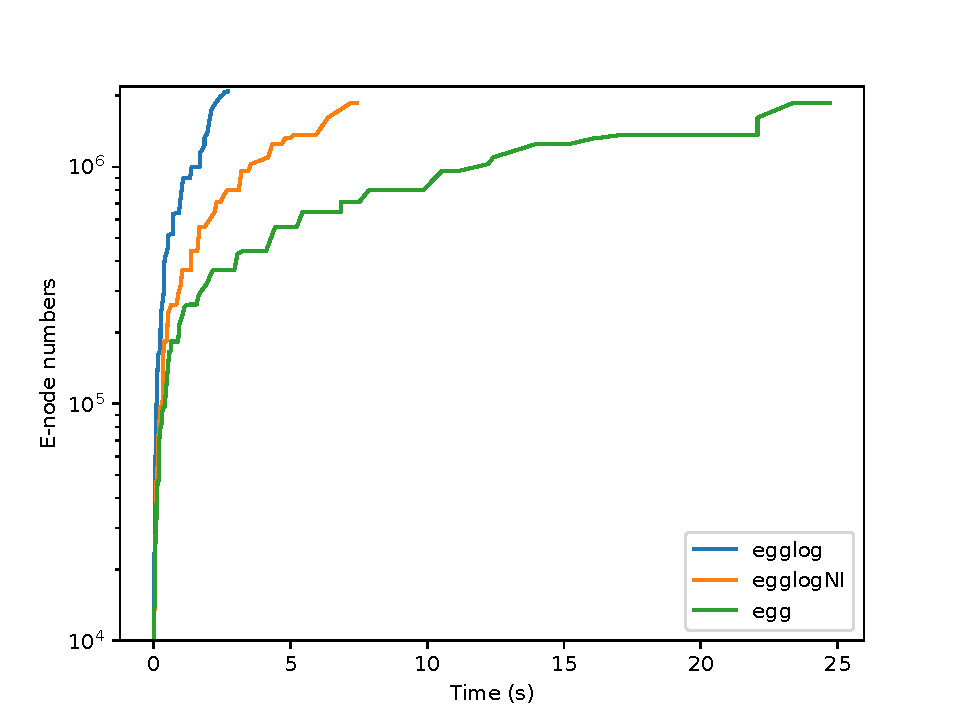
\includegraphics[width=0.5\textwidth]{figs/microbenchmarks.pdf}
        \caption{Performance of \egglog and \egg on \texttt{math} benchmark.
        \texttt{egglogNI} grows the same \egraph with less time than \egg.
        \egglog explores a larger program space 
        than both baselines thanks to semi-na\"ive evaluation.}
        \label{fig:microbenchmark}
    % \end{minipage}     
\end{figure}  
In this section, we evaluate the performance of \egglog
 on a typical workload of equality saturation.
Our two baselines are \egg, 
 a state-of-the-art equality saturation framework,
 and \texttt{egglogNI}, 
 the non-incremental variant of \egglog with \seminaive evaluation disabled.
We populate all three systems with a set of initial terms 
 from \egg's \texttt{math} test suite
 and grow the \egraph with rewrite rules using \texttt{BackOff} scheduler,
 the default scheduler of \egg.
We only use a subset of rules from \texttt{math} test suite that does not involve any analysis
 (so rules that require analyses like $x/x\rightarrow 1\text{ if } x\neq 0$ are removed),
 because the scheduler behaves differently on analyses in the two systems\footnote{
    \egglog does not distinguish analyses rules from other rules,
    while \egg treats \eclass analyses specially 
    and runs them to saturation in each iteration.
 }.
As a result,
 \texttt{egglogNI} and \egg produce the same \egraph in each iteration.

We ran each system for 100 iterations.\footnote{
    All experiments in this paper are executed on 
    a MacBook Pro with Apple M2 processor and 16GB memory.
}
For each iteration, 
 we ran three systems seven times and report the median time
 versus sizes of \texttt{math} \enodes (tuples for \egglog systems).
The result is shown in \autoref{fig:microbenchmark}.
Thanks to the efficient relational matching algorithm
 and the relational query optimizer, 
 \texttt{egglogNI} grows the exact same \egraph in less time 
 than \egg, yielding a 3.34$\times$ speedup at the end of iteration 100.
Moreover,
 \egglog grows a slightly larger e-graph than \egg with a 9.27$\times$ speedup,
 because its \seminaive evaluation avoids redundant matches.